\section{Demo}
\frame
{
\frametitle{Demo}
\begin{center}
 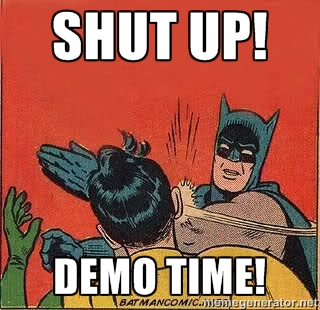
\includegraphics[height=4cm]{imgs/demo-time.jpg}
\end{center}

\begin{itemize}
 \item Crearemos nuestro propio repositorio Git en Bitbucket
 \item Crearemos nuestra rama de trabajo y subiremos cambios
 \item Propondremos la integración de estos cambios haciendo \textit{pull request}
 \item Simularemos la descarga del repositorio por parte de un compañero y subiremos nuevos cambios
 \item Actualizaremos el repo haciendo \textit{rebase} y subiremos más cambios
 \item Mostraremos cómo funciona el \textit{rebase} de manera gráfica
\end{itemize}
}
